\subsection{Te installeren software}

Volgende handleiding heeft de software gedeployed op een ubuntu distributie. Elk systeem (of distributie) die Glassfish, Java, Mariadb (of MySQL) en perl ondersteunt, kan gebruikt worden. De uitgevoerde commando's zullen echter verschillen. Werk je bijvoorbeeld op een centos of een fedora dan zal de apt-get packet manager niet werken en zal je yum moeten gebruiken.

Volgende zaken heb je nodig vanop je client systeem bij aanvang van de installatie:

\begin{itemize}
\item Terminal/console/putty/git bash die kan ssh'n naar de server.
\item Database dump in de vorm van een SQL-bestand (hier: verkeer.sql).
\item De pollservice die uitgevoerd wordt op de server (hier: verkeerPollService.jar)
\item De scrapers (hier: de map /scrapers/)
\item De webapplicatie die gedeployed wordt op glassfish (hier: verkeerweb.war)
\end{itemize}

Alle commando's die uitgevoerd opgesomd zijn, worden verondersteld uitgevoerd te worden op de ubuntu-server! Het SQL-bestand, de pollservice en de map /scrapers/ moeten op de server overgezet worden. Dit kan bijvoorbeeld via sftp of scp.

Een voorbeeld is:

\begin{lstlisting}[style=BashInputStyle]
	scp verkeer.sql root@x.y.z.q:/verkeer
	scp pollservice.jar root@x.y.z.q:/verkeer
	scp -r scrapers root@x.y.z.q:/verkeer/scrapers
\end{lstlisting}

\subsubsection{Datum/uur/tijdzone instellen}

\begin{lstlisting}[style=BashInputStyle]
	sudo timedatectl set-timezone Europe/Brussels
\end{lstlisting}

Een andere optie is via:

\begin{lstlisting}[style=BashInputStyle]
	apt-get install ntpdate
	dpkg-reconfigure tzdata
\end{lstlisting}





\subsubsection{Java 8 installeren}

\begin{lstlisting}[style=BashInputStyle]
	sudo add-apt-repository ppa:openjdk-r/ppa
	sudo apt-get update 
	sudo apt-get install openjdk-8-jdk -y
\end{lstlisting}

Controleren kan via:

\begin{lstlisting}[style=BashInputStyle]
	java -version
\end{lstlisting}

\subsubsection{Mariadb installeren}

\begin{lstlisting}[style=BashInputStyle]
	sudo apt-get install mariadb-server -y
\end{lstlisting}

Er zal gevraagd worden om een wachtwoord te kiezen voor mysql/mariadb.

\subsubsection{Extra tools installeren}

\begin{lstlisting}[style=BashInputStyle]
	sudo apt-get install unzip gcc make libjson-perl -y
\end{lstlisting}

Unzip gebruiken we om straks te unzippen. De c compiler, make hebben we nodig om de nodige zaken voor de scrapers te installeren.

\subsubsection{Glassfish installeren}

\begin{lstlisting}[style=BashInputStyle]
	wget http://download.oracle.com/glassfish/4.1/release/glassfish-4.1.zip
	unzip glassfish-4.1.1.zip -d /opt
	/opt/glassfish4/bin/asadmin start-domain
	/opt/glassfish4/bin/asadmin change-admin-password
	/opt/glassfish4/bin/asadmin enable-secure-admin
	/opt/glassfish4/bin/asadmin restart-domain
\end{lstlisting}

Met deze commando's doorloop je enkele stappen om een admin gebruiker te maken en het lege wachtwoord te wijzigen. Indien je vaak het asadmin programma gaat gebruiken dan kan het handig zijn om /opt/glassfish4/bin op te nemen in je PATH en dit toe te voegen aan je ~/.profile. Om een domein te stoppen gebruik je het commando ``asadmin stop-domain''.

\subsubsection{Perl installeren}

\begin{lstlisting}[style=BashInputStyle]
	sudo cpan JSON
	perl -MCPAN -e shell
		> install JSON::XS
\end{lstlisting}

\subsubsection{Mysql database verkeer in orde brengen}

\begin{lstlisting}[style=BashInputStyle]
	mysql -p
		create database verkeer;
		exit;
	mysql verkeer -u root < "verkeer.sql"
\end{lstlisting}

\subsubsection{Scrapers testen}

\begin{lstlisting}[style=BashInputStyle]
	root@server:~/scrapers# ./testscrapers.sh
\end{lstlisting}

Met dit scriptje worden alle scrapers getest. Op deze manier zien we of er data binnengehaald kan worden of niet.

\subsubsection{Poll service in een scriptje}

De poll service staat in dit voorbeeld in de root: /root/verkeerPollService.jar.
Met volgend script (runpollservice.sh) zorgen we ervoor dat hij automatisch herstart bij crashen:

\begin{lstlisting}[style=BashInputStyle]
	#!/bin/bash

	while true
	do
   		java -Xms256m -Xmx512m -jar VerkeerPollService.jar
  		#restart loop
   		sleep 5
	done
\end{lstlisting}

Het starten van de poll service gebeurt best in een screen:

\begin{lstlisting}[style=BashInputStyle]
	screen -S pollservice
	./runpollservice.sh
\end{lstlisting}

Met CTRL+A,D kan je het detachen.

\subsubsection{Instellen backup}

Volgende commando's voeren een script uit om een backup te maken aan de hand van een crontab.

\begin{lstlisting}[style=BashInputStyle]
	crontab -e
	#backup mysql db every midnight
	0 0 * * * /root/backupverkeer.sh
\end{lstlisting}

\subsubsection{Uploaden Verkeerweb}

Dit gebeurt in de browser door te surven naar glassfish. Deze is bereikbaar via http://server:4848. Inloggen doe je met de credentials die eerder werden ingesteld bij glassfish. Daarna kies je voor deploy application en kies je de war:

\begin{figure}[H]
\centering
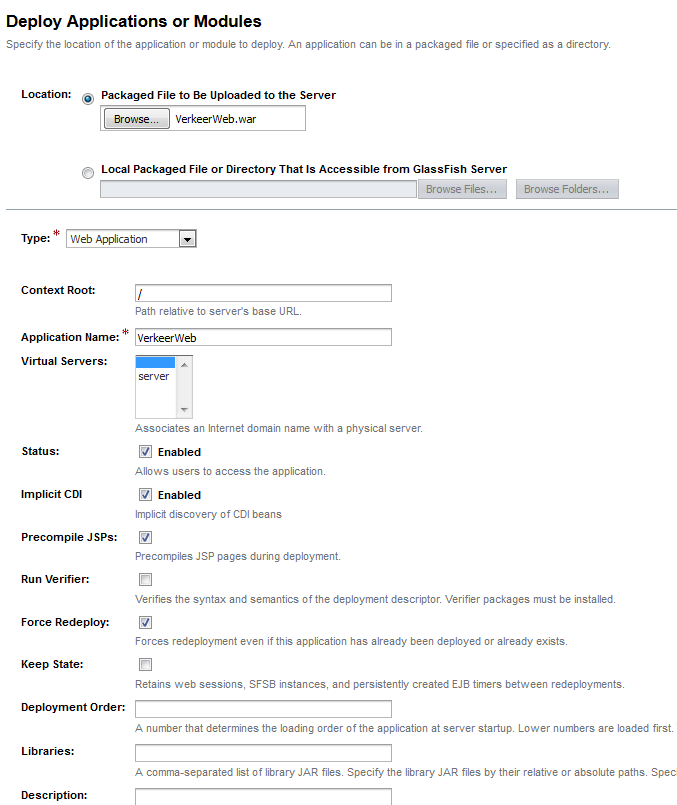
\includegraphics[width=\textwidth]{images/uploadverkeerweb.png}\\
\caption{Uploaden Verkeerweb}
\end{figure}